\documentclass[crop,tikz,border=10]{standalone}

\usepackage{amsmath, amssymb}
\usetikzlibrary{calc}
\usetikzlibrary{matrix}


\begin{document}
    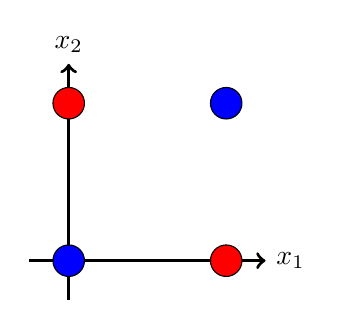
\begin{tikzpicture}
        \draw[very thick, ->] (0, -0.5) -- (0, 2.5) node[above] {$x_2$};;
        \draw[very thick, ->] (-0.5, 0) -- (2.5, 0) node[right] {$x_1$};;

        \draw[fill=blue] (0, 0) circle (0.2);
        \draw[fill=blue] (2, 2) circle (0.2);

        \draw[fill=red] (2, 0) circle (0.2);
        \draw[fill=red] (0, 2) circle (0.2);
    \end{tikzpicture}
\end{document}
